\section{Konsep Stream Cipher (Cipher Alir)}
\label{sec:konsep-stream-cipher}

\textit{Stream cipher} atau \textbf{cipher alir} adalah kategori cipher simetris
yang mengenkripsi plainteks satu satuan kecil pada satu waktu --- satu bit, satu
byte, atau $n$ bit --- dengan operasi XOR sebagai satu-satunya operasi
pencampurannya. Berbeda dengan cipher blok yang menunggu terkumpulnya satu blok
penuh sebelum bekerja, cipher alir memproses data begitu data itu tiba.

\subsection{Mekanisme Kerja}

Enkripsi pada cipher alir dilakukan dengan tiga cara yang ekuivalen, bergantung
pada satuan yang dipilih implementasinya:
\begin{itemize}
    \item $1$ bit plainteks di-XOR dengan $1$ bit kunci,
    \item $1$ byte plainteks di-XOR dengan $1$ byte kunci, atau
    \item $n$ bit plainteks di-XOR dengan $n$ bit kunci,
\end{itemize}
setiap kali enkripsi dilakukan. Dekripsi memakai aturan yang persis sama,
dengan cipherteks menggantikan plainteks.

Inti dari cipher alir adalah \textbf{\textit{keystream generator}}. Generator
ini menerima kunci rahasia (dan seringkali sebuah \textit{Initialization Vector}
atau IV) sebagai \textit{seed}, lalu membangkitkan aliran bit acak yang
panjangnya sama dengan pesan. Aliran itulah yang disebut \textbf{\textit{keystream}}
atau kunci-alir. Bit-bit keystream di-XOR-kan dengan bit-bit plainteks pada
posisi yang bersesuaian,
\begin{equation}
c_i = p_i \oplus k_i,
\label{eq:stream-enkripsi}
\end{equation}
dan di sisi penerima keystream yang sama dibangkitkan ulang untuk mengembalikan
plainteks,
\begin{equation}
p_i = c_i \oplus k_i.
\label{eq:stream-dekripsi}
\end{equation}
Susunan pengirim, penerima, dan keystream generator diperlihatkan pada
Gambar~\ref{fig:diagram-blok-stream-cipher}.

\begin{figure}[htbp]
    \centering
    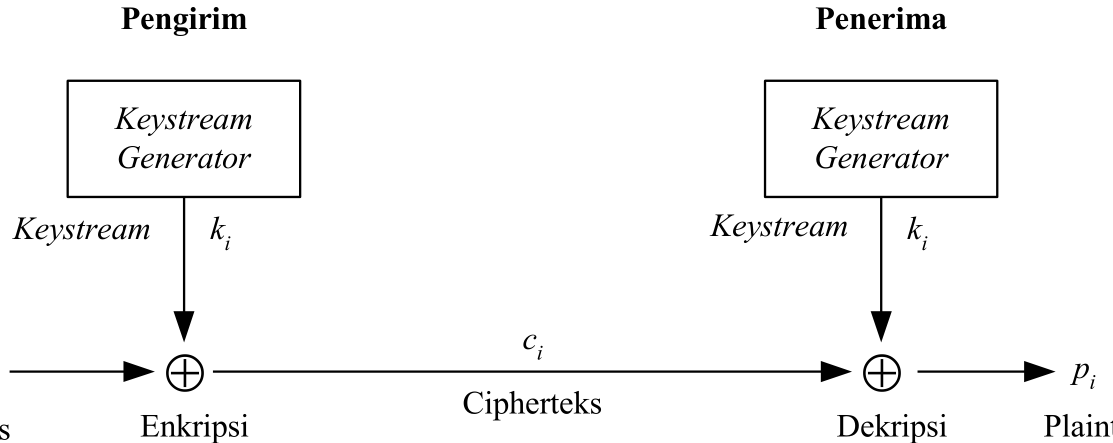
\includegraphics[width=0.9\linewidth, height=0.7\textheight, keepaspectratio]{figures/diagram-blok-stream-cipher.png}
    \caption{Diagram blok cipher alir: pengirim dan penerima membangkitkan keystream yang sama, lalu keystream di-XOR dengan plainteks saat enkripsi dan dengan cipherteks saat dekripsi}
    \label{fig:diagram-blok-stream-cipher}
    \sumber{Munir, \textit{IF4020 Kriptografi}, ITB.}
\end{figure}

\subsection{Keystream Generator dan Umpan}

Karena tidak mungkin mengirimkan kunci sepanjang pesan melalui saluran yang
sama dengan pesannya, keystream harus dibangkitkan. Keystream generator
diimplementasikan sebagai prosedur yang sama di sisi pengirim maupun penerima.
Prosedur itu menerima sebuah umpan (\textit{seed}) $U$ dan keluarannya merupakan
fungsi dari $U$; pengirim dan penerima harus memiliki umpan yang sama, dan umpan
itu harus dijaga kerahasiaannya karena kedudukannya setara dengan kunci
eksternal. Generator dapat membangkitkan keystream dalam satuan bit, byte, atau
blok bit.

Bit-bit keystream bersifat acak, tetapi bukan acak sejati (\textit{true random})
melainkan \textbf{acak semu} (\textit{pseudo-random}). Bedanya penting: bit acak
sejati tidak dapat dibangkitkan ulang, sedangkan bit acak semu dapat
dibangkitkan ulang secara identik asalkan umpan $U$ yang dipakai sama. Sifat
inilah yang memungkinkan penerima mendekripsi pesan. Sebagai konsekuensinya,
barisan bit acak semu selalu memiliki \textbf{periode}: setelah sejumlah iterasi
tertentu barisan itu terulang kembali.

Periode menjadi ukuran keamanan yang pertama. Bila periode keystream lebih
pendek daripada pesan, maka bit kunci akan dipakai ulang di dalam satu pesan
yang sama --- persis situasi yang pada Bab~\ref{chap:kriptografi-klasik} membuat
Vigen\`ere cipher dapat dipecahkan dengan metode Kasiski. Karena itu perancang
cipher alir berusaha membuat periode keystream sangat panjang, misalnya dengan
menggabungkan beberapa register atau memberi umpan balik non-linier. Register
berukuran $n$ bit dapat memberi periode maksimum $2^n - 1$ bit, sehingga register
32 bit memberi periode lebih dari empat miliar bit.

Keamanan yang kedua adalah \emph{ketidakterulangan pemakaian}. Umpan $U$ hanya
boleh dipakai sekali untuk satu pesan. Bila umpan yang sama dipakai dua kali,
dua cipherteks akan memakai keystream yang identik dan kunci saling menghapus
saat keduanya di-XOR, seperti yang ditunjukkan pada Bagian~\ref{sec:kriptografi-modern}.
Untuk menghindari hal itu, cipher alir modern memisahkan peran kunci dan umpan:
kunci tetap rahasia dan dipakai berulang, sedangkan \textit{nonce}
(\textit{number used once}) berubah untuk setiap pesan. Dengan cara ini keystream
yang dibangkitkan selalu berbeda meskipun kuncinya sama.

\subsection{Umpan Balik dan LFSR}

Contoh paling klasik dari keystream generator adalah \textbf{\textit{Feedback
Shift Register}} (FSR). FSR terdiri atas dua bagian: sebuah register geser
sepanjang $n$ bit dan sebuah fungsi umpan balik. Setiap kali detak diberikan,
isi register bergeser satu posisi dan bit yang paling ujung terlempar keluar
menjadi bit keystream. Bit keluaran itu juga menjadi masukan bagi fungsi umpan
balik yang menghitung bit baru untuk mengisi posisi yang kosong. Skemanya
diperlihatkan pada Gambar~\ref{fig:fsr-blok}.

\begin{figure}[htbp]
    \centering
    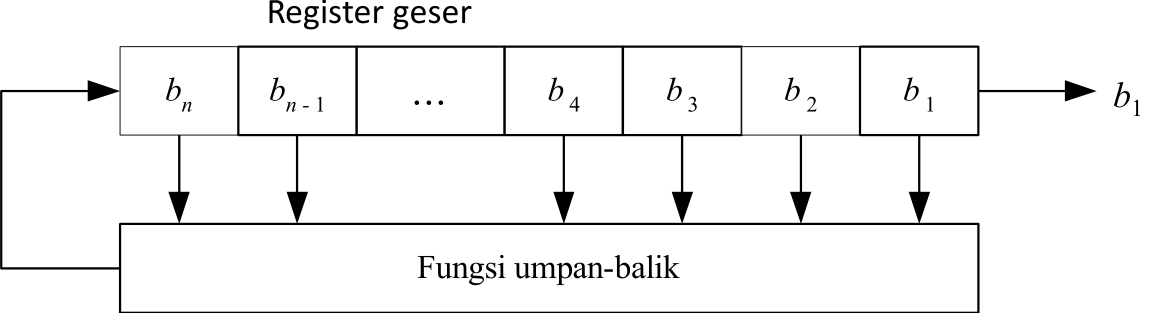
\includegraphics[width=0.8\linewidth, height=0.3\textheight, keepaspectratio]{figures/fsr-blok.png}
    \caption{Register geser dengan fungsi umpan balik: bit yang terlempar keluar menjadi bit keystream, dan sebagian bit register diumpanbalikkan untuk mengisi posisi yang kosong}
    \label{fig:fsr-blok}
    \sumber{Munir, \textit{IF4020 Kriptografi}, ITB.}
\end{figure}

Bila fungsi umpan baliknya hanya melibatkan operasi XOR, FSR itu disebut
\textbf{\textit{Linear Feedback Shift Register}} (LFSR). Misalkan bit-bit
register dinyatakan sebagai $b_n b_{n-1} \dots b_1$; pada setiap detak, bit
$b_n$ bergeser ke tempat $b_{n-1}$, $b_{n-1}$ bergeser ke $b_{n-2}$, dan
seterusnya, sedangkan $b_1$ terlempar keluar dan menjadi bit luaran. Posisi $b_n$
yang kosong kemudian diisi dengan
\[
b_n = b_1 \oplus b_2 \oplus \dots \oplus b_{n-1} \oplus b_n ,
\]
yaitu XOR dari bit-bit yang dipilih oleh \emph{tap} (\textit{titik sadap}).
Gambar~\ref{fig:lfsr} memperlihatkan LFSR 4 bit dengan dua tap.

\begin{figure}[htbp]
    \centering
    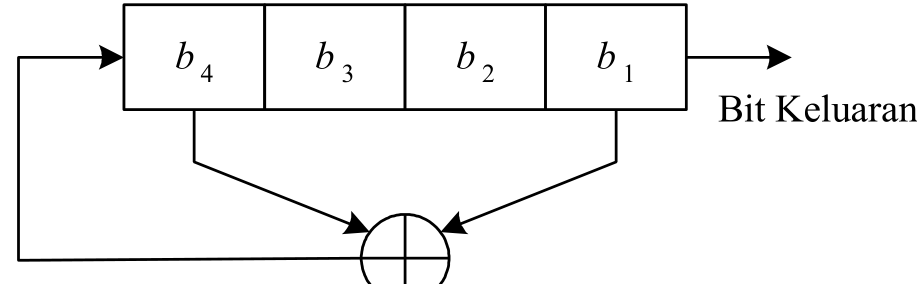
\includegraphics[width=0.72\linewidth, height=0.6\textheight, keepaspectratio]{figures/lfsr.png}
    \caption{Diagram blok LFSR 4 bit; bit keluaran sekaligus menjadi umpan balik melalui gerbang XOR dari dua tap}
    \label{fig:lfsr}
    \sumber{Munir, \textit{IF4020 Kriptografi}, ITB.}
\end{figure}

Sebagai contoh terhitung, ambil LFSR 4 bit dengan isi awal $U = \code{1111}$ dan
umpan balik $f = b_3 \oplus b_0$, yaitu tap pada bit paling kiri dan paling
kanan. Register bergeser ke kanan satu bit setiap detak, bit keluaran adalah
$b_0$, dan bit $f$ masuk ke posisi $b_3$. Perubahan isi register dan bit
keluarannya diperlihatkan pada Tabel~\ref{tab:lfsr-4bit}.

\begin{table}[htbp]
\centering
\small
\begin{tabular}{@{}c c c c c c@{}}
\hline
$i$ & $b_3$ & $b_2$ & $b_1$ & $b_0$ & Keluaran \\
\hline
0  & 1 & 1 & 1 & 1 & 1 \\
1  & 0 & 1 & 1 & 1 & 1 \\
2  & 1 & 0 & 1 & 1 & 1 \\
3  & 0 & 1 & 0 & 1 & 1 \\
4  & 1 & 0 & 1 & 0 & 0 \\
5  & 1 & 1 & 0 & 1 & 1 \\
6  & 0 & 1 & 1 & 0 & 0 \\
7  & 0 & 0 & 1 & 1 & 1 \\
8  & 1 & 0 & 0 & 1 & 1 \\
9  & 0 & 1 & 0 & 0 & 0 \\
10 & 0 & 0 & 1 & 0 & 0 \\
11 & 0 & 0 & 0 & 1 & 1 \\
12 & 1 & 0 & 0 & 0 & 0 \\
13 & 1 & 1 & 0 & 0 & 0 \\
14 & 1 & 1 & 1 & 0 & 0 \\
\hline
\end{tabular}
\caption{Isi register dan bit keluaran LFSR 4 bit bermuatan awal \code{1111} dengan umpan balik $f=b_3\oplus b_0$}
\label{tab:lfsr-4bit}
\sumber{Data dari Munir, \textit{IF4020 Kriptografi}, ITB; tabel dihitung ulang dari aturan umpan balik tersebut.}
\end{table}

\noindent
Sebagai ilustrasi langkah $i=0 \to 1$: karena $f = 1 \oplus 1 = 0$ dan bit
keluarannya $b_0 = 1$, register $1111$ berubah menjadi $0111$. Barisan bit
keluaran yang terbentuk adalah
\begin{center}
\texttt{111101011001000}
\end{center}
dan setelah 15 detak register kembali ke keadaan semula, yaitu $1111$. Jadi
periode LFSR 4 bit ini adalah $2^4 - 1 = 15$ bit, bukan $16$ bit, karena keadaan
register $0000$ akan membuat seluruh register bernilai nol selamanya. Secara
umum, LFSR $n$ bit dapat mencapai periode maksimum $2^n - 1$ bila polinomial
umpan baliknya dipilih dengan tepat (polinomial primitif).

Meski cepat dan hemat perangkat keras, LFSR tunggal \emph{tidak aman} untuk
kriptografi. Keluarannya bersifat linier terhadap keadaan awal, sehingga dengan
menyadap sekitar $2n$ bit keluaran seorang penyerang dapat menyusun sistem
persamaan linier dan memulihkan seluruh tap beserta keadaan awal register tanpa
pencarian menyeluruh; prosedur sistematis untuk itu, yaitu algoritma
Berlekamp--Massey, sudah dikenal sejak akhir dekade 1960-an
\citep{massey1969}. Karena itu cipher alir praktis tidak pernah memakai satu
LFSR saja, melainkan menggabungkan beberapa register melalui fungsi non-linier:
A5/1 memakai tiga LFSR dengan kaidah detak mayoritas, sedangkan Trivium memakai
tiga register umpan balik non-linier (NLFSR). Keduanya dibahas pada
Bagian~\ref{sec:algoritma-stream-cipher}.

\subsection{Penyebaran Galat dan Aplikasi Cipher Alir}

Ciri khas cipher alir adalah \textbf{melokalisasi galat}. Karena setiap bit
plainteks ditentukan hanya oleh satu bit cipherteks dan satu bit keystream,
kesalahan satu bit pada cipherteks menghasilkan kesalahan tepat satu bit pada
plainteks hasil dekripsi --- tidak menyebar seperti pada cipher blok dengan
mode rantai. Sifat ini diperlihatkan oleh contoh terhitung pada
Tabel~\ref{tab:galat-cipher-alir}.

\begin{table}[htbp]
\centering
\small
\begin{tabular}{@{}l @{\hspace{10pt}} l@{}}
\hline
Plainteks $P$      & \texttt{0101 0111 0001 1001 0110 0100} \\
Keystream $K$      & \texttt{1111 0101 1001 0001 1110 1011} \\
\hline
Cipherteks $C$     & \texttt{1010 0010 1000 1000 1000 1111} \\
Cipherteks rusak   & \texttt{1010 1010 1000 1000 1000 1111} \\
\hline
Dekripsi $C$       & \texttt{0101 0111 0001 1001 0110 0100} \\
Dekripsi $C$ rusak & \texttt{0101 1111 0001 1001 0110 0100} \\
\hline
\end{tabular}
\caption{Galat satu bit pada cipherteks cipher alir hanya merusak satu bit plainteks. Bit ke-5 cipherteks diubah dari $0$ menjadi $1$, dan bit ke-5 plainteks ikut berubah}
\label{tab:galat-cipher-alir}
\sumber{Data dari Munir, \textit{IF4020 Kriptografi}, ITB; perhitungan XOR diulang untuk memastikan hasilnya.}
\end{table}

Sifat melokalisasi galat itu punya dua sisi. Di satu pihak, ia menguntungkan
untuk saluran komunikasi yang bising: satu bit yang rusak dalam perjalanan
tidak merusak bit-bit berikutnya, sehingga suara pada sambungan telepon tetap
terdengar wajar meskipun sesekali ada bit yang salah. Di pihak lain, sifat itu
membuka pintu bagi serangan \textit{flip-bit}: penyerang yang mengetahui makna
sebuah bit pada posisi tertentu dapat membalik bit itu pada cipherteks dan
mengubah plainteks dengan cara yang dapat diduga, tanpa pernah mengetahui
kuncinya. Karena itu cipher alir tidak memberi jaminan keutuhan data;
keutuhan harus ditambahkan melalui kode otentikasi pesan
(Bab~\ref{chap:hash-mac}).

Dengan sifat-sifat di atas, cipher alir cocok dipakai untuk mengenkripsi aliran
data yang kontinu melalui saluran komunikasi, misalnya pada sambungan antara
dua komputer dan pada transmisi suara jaringan telepon seluler GSM. Alasannya
ada tiga: komputasinya sangat cepat sehingga cocok untuk pemrosesan
\textit{real-time}, galat tidak menyebar, dan tidak ada penundaan akibat
menunggu terkumpulnya satu blok penuh. Sebaliknya, cipher alir kurang cocok
untuk data yang perlu diakses secara acak (\textit{random access}) seperti berkas
pada penyimpanan, karena keystream harus dibangkitkan dari awal. Keterbatasan
itu diatasi oleh cipher alir modern yang memakai pencacah (\textit{counter}),
sehingga blok keystream pada posisi mana pun dapat dihitung langsung.

\subsection{Stream Cipher vs Block Cipher}

Perbedaan kedua kategori cipher simetris ini diringkas pada
Tabel~\ref{tab:stream-vs-block}.

\begin{table}[htbp]
\centering
\small
\begin{tabularx}{\linewidth}{@{}>{\raggedright\arraybackslash}p{3.0cm} >{\raggedright\arraybackslash}X >{\raggedright\arraybackslash}X@{}}
\hline
\textbf{Aspek} & \textbf{Stream Cipher} & \textbf{Block Cipher} \\
\hline
Satuan pemrosesan & 1 bit, 1 byte, atau $n$ bit per langkah & Satu blok tetap, misalnya 128 bit \\
\hline
Operasi pencampur & XOR dengan keystream & Substitusi, permutasi, dan putaran berlapis \\
\hline
Kebutuhan memori & Kecil; hanya keadaan internal generator & Lebih besar; perlu penyangga satu blok \\
\hline
Panjang keluaran & Sepanjang pesan, tanpa penambahan bit & Kelipatan ukuran blok; perlu \textit{padding} \\
\hline
Penyebaran galat & Tidak menyebar; 1 bit rusak $\rightarrow$ 1 bit rusak & Menyebar ke seluruh blok atau antar blok \\
\hline
Akses acak & Umumnya berurutan, kecuali yang berbasis pencacah & Dapat diakses per blok \\
\hline
Penggunaan khas & Suara GSM, sambungan data kontinu, TLS dengan ChaCha20 & Berkas, basis data, disk, TLS dengan AES \\
\hline
Contoh algoritma & RC4, A5/1, Trivium, Salsa20, ChaCha20 & DES, AES, Blowfish, Twofish \\
\hline
\end{tabularx}
\caption{Perbandingan stream cipher dan block cipher}
\label{tab:stream-vs-block}
\sumber{Data dari Munir, \textit{IF4020 Kriptografi}, ITB; tabel disusun dari uraian tersebut beserta \citet{stallings2017}.}
\end{table}

Dari tabel itu terlihat bahwa pilihan antara keduanya bukan soal mana yang
lebih kuat, melainkan soal kesesuaian dengan kebutuhan. Cipher alir menang pada
kecepatan dan kelambanan rendah; cipher blok menang pada fleksibilitas pemakaian
ulang dan pada kemudahan menambahkan mode operasi. Bagian berikutnya membahas
empat cipher alir yang mewakili perkembangan gagasan selama lebih dari tiga
dasawarsa, dari RC4 yang lahir 1987 sampai ChaCha20 yang dipakai TLS 1.3.
